% AY2015 力学 第1問 転記（問題のみ）
\section*{第1問〔I〕}

次の問い〔I〕および〔II〕に答えよ。なお，〔I〕の解答は解答用紙 (1) に，
〔II〕の解答は解答用紙 (2) に記入せよ。

\medskip
図1に示すように，半径が $a$，質量が $M$，慣性モーメントが $\dfrac{2}{5}Ma^2$ で，
密度が一様な剛体球が傾斜角 $\theta$ の斜面を角速度 $\omega(t)$ で回転しながら落ちている。
このとき，剛体球と斜面との接地点にはすべりはなく，摩擦力 $f$ が働いている。
ここで，重力加速度を $g$，剛体球の重心を $G$ とし，$xy$ 座標を図1のようにとる。
このとき，次の問い (1)〜(6) に答えよ。

\begin{enumerate}[label=(\arabic*)]
  \item 剛体球に働く $x$ 方向の力を求めよ。
  \item 重心 $G$ の $x$ 方向の速度を $V$ とし，重心 $G$ の並進運動に関する
        $x$ 方向の運動方程式を求めよ。
  \item 摩擦力 $f$ によって，剛体球に働くトルクの大きさを求めよ。
  \item 剛体球の回転運動に関する運動方程式を求めよ。
  \item 重心 $G$ の並進運動に関する $x$ 方向の加速度を求めよ。ただし，摩擦力 $f$ に
        ついては上記の問いで求めた式を用いること。
  \item 重心 $G$ の並進運動に関する $x$ 方向の加速度を $A_1$，同じ斜面で摩擦のない
        場合の質点の $x$ 方向の加速度を $A_2$ として，加速度の比 $A_1/A_2$ を求めよ。
\end{enumerate}

\begin{center}
% 図1：傾斜角θの斜面を転がり落ちる剛体球。x軸=斜面下り方向、y軸=斜面法線
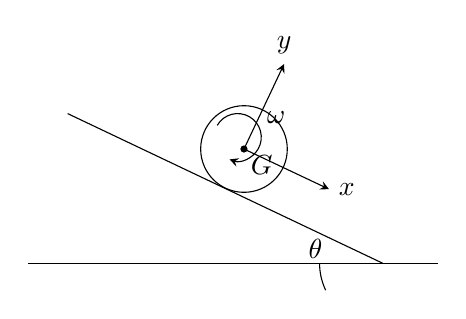
\begin{tikzpicture}[>=stealth, scale=1.0]
  \draw (-0.2,0) -- (5.0,0);                       % 水平地面
  \draw (0.3,1.9) -- (4.3,0);                      % 斜面
  \draw (3.5,0) arc (180:205.4:0.8); \node at (3.45,0.18) {$\theta$};
  % 球（斜面に接する）
  \coordinate (Gc) at (2.54,1.45);
  \draw (Gc) circle (0.55);
  \fill (Gc) circle (1.3pt); \node[below right=-1pt] at (Gc) {$G$};
  % 角速度ω
  \draw[->] (2.2,1.75) arc (150:-110:0.3); \node at (2.95,1.85) {$\omega$};
  % 座標軸（x:斜面下り、y:斜面法線）
  \draw[->] (Gc) -- ++(1.08,-0.51) node[right] {$x$};
  \draw[->] (Gc) -- ++(0.51,1.08) node[above] {$y$};
\end{tikzpicture}

{\small 図 1\quad 剛体球の運動}
\end{center}
